\documentclass[a4paper,12pt]{report}

\usepackage[utf8x]{inputenc}
\usepackage[T2A]{fontenc}
\usepackage[english, russian]{babel}

% Опционно, требует  apt-get install scalable-cyrfonts.*
% и удаления одной строчки в cyrtimes.sty
% Сточку не удалять!
% \usepackage{cyrtimes}

% Картнки и tikz
\usepackage{graphicx}
\usepackage{tikz}
\usetikzlibrary{snakes,arrows,shapes}


% Увы, поля придётся уменьшить из-за листингов.
\topmargin -1cm
\oddsidemargin -0.5cm
\evensidemargin -0.5cm
\textwidth 17cm
\textheight 24cm

\sloppy



% Оглавление в PDF
\usepackage[
bookmarks=true,
colorlinks=true, linkcolor=black, anchorcolor=black, citecolor=black, menucolor=black,filecolor=black, urlcolor=black,
unicode=true
]{hyperref}

% Для исходного кода в тексте
% \newcommand{\Code}[1]{\texttt{#1}}

% Некоторая русификация.
% \usepackage{misccorr} % Oh shi^W^W, оно не работает с report.
\usepackage{indentfirst}
\renewcommand{\labelitemi}{\normalfont\bfseries{--}}

% На дворе XXI век, но пакет listings всё ещё не пашет с русскими комментариями!

% Пакет listings для простой вставки исходников
% \usepackage{listings}
% Параметры оформления
% \lstset{
% showspaces=false,
% showtabs=false,
% frame=single,
% tabsize=4,
% basicstyle=\ttfamily,
% identifierstyle=\ttfamily,
% commentstyle=\itshape,
% stringstyle=\ttfamily,
% keywordstyle=\ttfamily,
% breaklines=true
% }
% Русский в комментариях.
% \lstset{escapebegin=\begin{cyr},escapeend=\end{cyr}}



% А это взято из файла, сгенерённого doxygen
% \usepackage{calc}
% \usepackage{array}
% \newenvironment{Code}
% {\footnotesize}
% {\normalsize}
% \newcommand{\doxyref}[3]{\textbf{#1} (\textnormal{#2}\,\pageref{#3})}
% \newenvironment{DocInclude}
% {\footnotesize}
% {\normalsize}
% \newenvironment{VerbInclude}
% {\footnotesize}
% {\normalsize}
% \newenvironment{Image}
% {\begin{figure}[H]}
% {\end{figure}}
% \newenvironment{ImageNoCaption}{}{}
% \newenvironment{CompactList}
% {\begin{list}{}{
%   \setlength{\leftmargin}{0.5cm}
%   \setlength{\itemsep}{0pt}
%   \setlength{\parsep}{0pt}
%   \setlength{\topsep}{0pt}
%   \renewcommand{\makelabel}{\hfill}}}
% {\end{list}}
% \newenvironment{CompactItemize}
% {
%   \begin{itemize}
%   \setlength{\itemsep}{-3pt}
%   \setlength{\parsep}{0pt}
%   \setlength{\topsep}{0pt}
%   \setlength{\partopsep}{0pt}
% }
% {\end{itemize}}
% \newcommand{\PBS}[1]{\let\temp=\\#1\let\\=\temp}
% \newlength{\tmplength}
% \newenvironment{TabularC}[1]
% {
% \setlength{\tmplength}
%      {\linewidth/(#1)-\tabcolsep*2-\arrayrulewidth*(#1+1)/(#1)}
%       \par\begin{tabular*}{\linewidth}
%              {*{#1}{|>{\PBS\raggedright\hspace{0pt}}p{\the\tmplength}}|}
% }
% {\end{tabular*}\par}
% \newcommand{\entrylabel}[1]{
%    {\parbox[b]{\labelwidth-4pt}{\makebox[0pt][l]{\textbf{#1}}\vspace{1.5\baselineskip}}}}
% \newenvironment{Desc}
% {\begin{list}{}
%   {
%     \settowidth{\labelwidth}{40pt}
%     \setlength{\leftmargin}{\labelwidth}
%     \setlength{\parsep}{0pt}
%     \setlength{\itemsep}{-4pt}
%     \renewcommand{\makelabel}{\entrylabel}
%   }
% }
% {\end{list}}
% \newenvironment{Indent}
%   {\begin{list}{}{\setlength{\leftmargin}{0.5cm}}
%       \item[]\ignorespaces}
%   {\unskip\end{list}}



\title{Рассчётно-пояснительная записка по курсовой работе "Разработка почтового сервера"}
\author{Кисленко Максим Германович}

\begin{document}

\maketitle

\tableofcontents

\cleardoublepage
\phantomsection
\addcontentsline{toc}{chapter}{Введение}
\chapter*{Введение}

% Два предложения о содержании отчёта. Для нового абзаца в исходном тексте должна быть пустая строка.

% Это~-- шаблон отчёта (вот как оформляется длинное тире, перед котрым идёт неразрывный пробел).

Курсовая работа предполагает разработку собственного почтового сервера, который будет использоваться для пересылки электронных писем (email-ов) в IP-сети. Вся работа поделена на две приблизительно одинаковые части - разработка почтового сервера, осуществляющего приём писем, и разработка почтового клиента, который переотправит письма другим почтовым серверам в зависимости от получателей-адресатов. Эти части разрабатываются независимо друг от друга двумя студентами, а потом интегрируются в единую систему. Команде студентов дополнительно присваивается вариант, который определяет основные требования к реализации или функциональности.

При реализации подразумевается, что используются низкоуровневые системные вызовы и, что сервер работает под управлением POSIX-совместимой операционной системы. Последнее условие необходимо, чтобы обеспечить переносимость созданного ПО.

В данном документе будет рассмотрена разработка почтового сервера, с условиями от варианта 12. Условия включают в себя следующие пункты:
\begin{itemize}
	\item сервер должен обрабатывать входящие соединения в единственном рабочем потоке с применением вызова poll. Такое условие подразумевает использование сокетов в режиме неблокирующего ввода-вывода, так как иначе, единственный поток бы блокировался на одном клиенте и не мог бы считаться полноценным сервером;
	\item логирование событий и ошибок в работе сервера должно происходить в отдельном процессе. Такое техническое решение увеличивает сложность реализации, но и делает сервер более производительным (отсутствуют операции ввода-вывода на жесткий диск);
	\item проверка обратной зоны dns не предполагается.
\end{itemize}
Независимо от условий варианта, при постановке задачи заданы требования к выполнению данной работы. А именно:
\begin{itemize}
	\item в качестве протокола пересылки электронных сообщений предписано использовать протокол SMTP (simple mail transfer protocol). Вся необходимая информация по нему доступна в RFC 5321;
	\item для локального хранения писем использовать механизм Maildir;
	\item конфигурация сервера должна быть вынесена в отдельный конфигурационный файл;
	\item необходимо разработать автоматическое тестирование созданного ПО (системные, unit-тесты);
	\item необходимо автоматизировать сборку проекта из исходников.
\end{itemize}

В поставленной задаче довольно жестко регламентированы используемые технологии. В качестве основного языка программирования - язык Си стандарта 99-го года. Для автоматизации тестирования - cunit или скриптовые языки (python, ruby или другое). Для автоматизации сборки - только GNU Make. Также готовое ПО необходимо протестировать на наличие утечек памяти с помощью утилиты valgrind.

Готовая программа должна обрабатывать входящие соединения, обслуживать их в соответствии с правилами сессии SMTP, сохранять письма локально в Maildir вместе с необходимыми заголовками, и передавать письма на дальнейшую отправку SMTP-клиенту. Далее в этом документе детально рассмотрены:

\begin{itemize}
	\item Пользовательское взаимодействие с сервером, его достоинства, недостатки и существующие аналоги в аналитическом разделе;
	\item Проектирование и принятые программные решения при создании ПО в конструкторском разделе;
	\item Используемые инструменты и технологии, порядок эксплуатации созданного ПО в технологическом разделе;
\end{itemize}

% А вот так оформляются списки: \begin{itemize} \item элемент списка; \item последний элемент списка. \end{itemize}

% Нумерованный список выглядит следующим образом. \begin{enumerate} \item Первый элемент. \item Второй элемент. \end{enumerate}


\chapter{Аналитический раздел}

\section{Предметная область}

В результате проведённого исследования были выделены следующие сущности предметной области (рисунок ~\ref{fig:entities}). Здесь и далее все диаграммы выполняются в нотациях UML, если иное не указано явно.

\begin{figure}
\centering
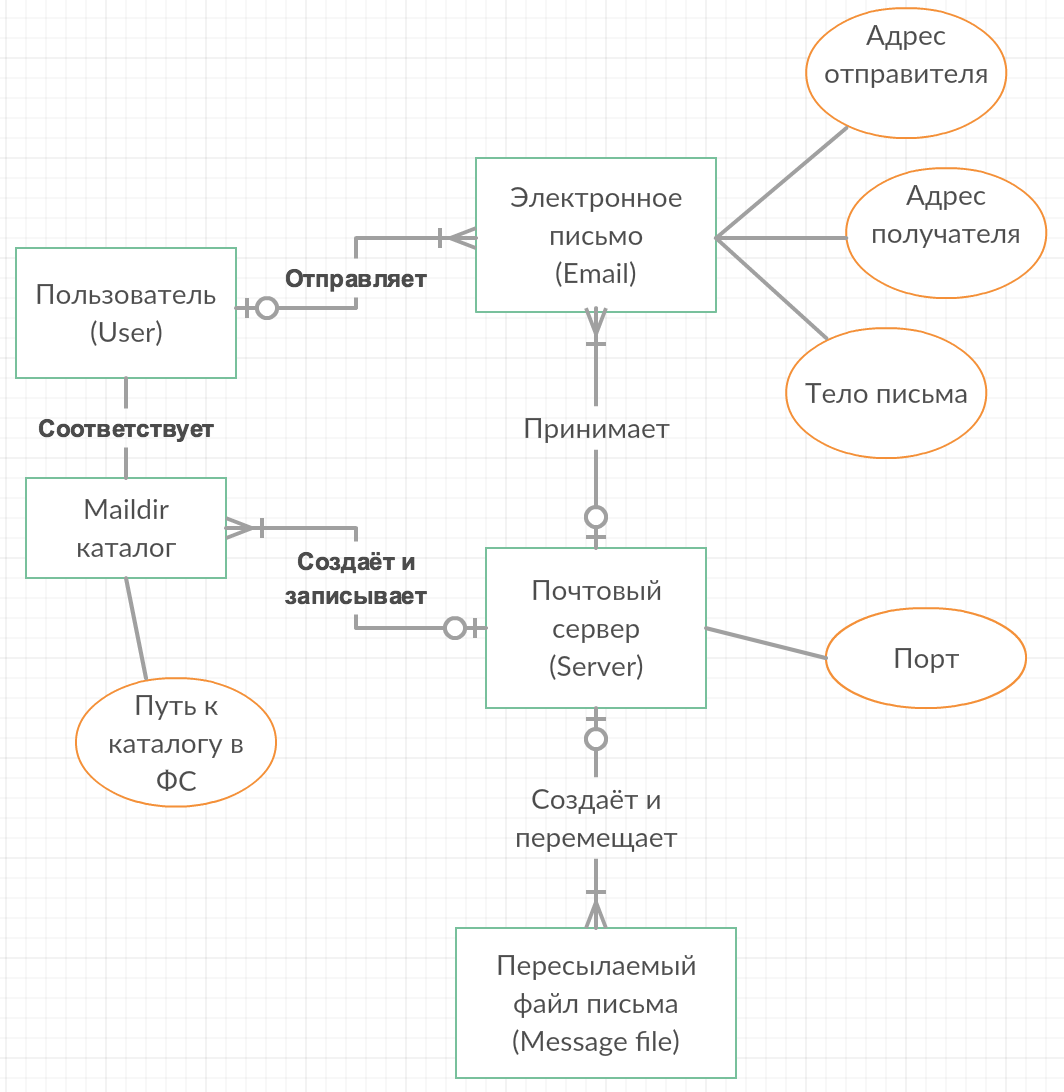
\includegraphics[width=\textwidth]{diagramms/entities.png}
\caption{Основные сущности предметной области}
\label{fig:entities}
\end{figure}


\section{Сценарии работы с SMTP-сервером}

\section{Достоинства и недостатки реализуемого сервера}

\section{Программы аналоги}


\chapter{Конструкторский раздел}

\section{Архитектура сервера}

Реализация почтового сервера разделена на несколько функциональных модулей с собственными заголовочными файлами. В server.h и server.c выполняется установка соединений с клиентами, получение от них текстовых команд и вызов SMTP-парсера для формирования ответа. Он также хранит для каждого из соединений запись о текущем состоянии (это связано с тем, что SMTP является stateful-протоколом). Сервер является однопроцессным, однопоточным и работает с сокетами клиентов в режиме неблокирующего ввода-вывода. Для получения событий о готовности ввода-вывода применяется системный вызов \textit{poll()}. Подобная архитектура применяется в http-серверах nginx (с процессами-воркерами для обработки запросов) и node.js.

Опишем алгоритм работы сервера с помощью python-подобного псевдокода. Пусть \textit{fd} будет основным сокетом, на котором сервер сделал вызовы \textit{bind()} и \textit{listen()}, тогда:

\begin{verbatim}
sockets = []
sockets.append({fd: fd, events: POLLIN})
active_cnt = 1

while True:
    code = poll(sockets, active_cnt, timeout)
    if code == 0:
        # timeout expired
        return 0

    quit = []
    for sock in sockets:
        if sock == fd:
            accept_new_conns(fd)
        else:
            state = get_state(sock)
            code = handle_known_conn(state) 
            if code < 0:
                # received QUIT command
                quit.append(sock)

    if quit:
        for sock in quit:
            sockets.remove(sock)
\end{verbatim}

Здесь и далее в листингах не показываются обработки ошибок, только основные действия. Чтобы принять новые соединения сервер выполняет внутри функции \textit{accept_new_conns} системный вызов \textit{accept}.

\begin{verbatim}
while True:
    new_sock = accept(fd)
    if new_sock < 0:
        return new_sock
    else:
        create_state(new_sock)
        send(new_sock, 'Welcome!')

        sockets.append(new_sock)
        active_cnt += 1
\end{verbatim}

Если поступают данные от клиента, то сервер вызовет \textit{handle_new_conn}, предварительно восстановив состояние этого клиента по сокету. Для получения данных используется вызов \textit{recv}. Для анализа полученных от клиента данных функция SMTP-парсера \textit{handle_request}.

\begin{verbatim}
input = ''

while True:
    chunk = recv(sock, input, 1000)
    if chunk:
        input += chunk
    else:
        break

if input:
    resp = handle_request(input)
    send(sock, resp)

\end{verbatim}

% Рис.~\ref{fig:fsm} нагенерил самодельный \textit{fsm2dot} из \textit{autogen} и \textit{dot2tex} на пару \textit{dot}. Никто не мешает изменить параметры типа \textit{rankdir} прямо в \textit{fsm2dot}, если он будет лучше смотреться, например, сверху-вниз.

% \begin{figure} \centering \includegraphics[width=\textwidth]{include/server_def_dot.pdf} \caption{Состояния сервера} \label{fig:fsm} \end{figure}

\section{Обработка команд протокола}

Далее SMTP-парсер, анализирует полученную строку и в зависимости от неё и текущего состояния конкретного клиента выбирает выполняемое действие, новое состояние и нужный ответ клиенту. Парсер реализован в отдельном модуле из файлов smtp.h и smtp.c. По сути он представляет собой конечный автомат и может быть описан диаграммой состояний переходов (рисунок ~\ref{fig:smtp_fsm}).

\begin{figure}
\centering
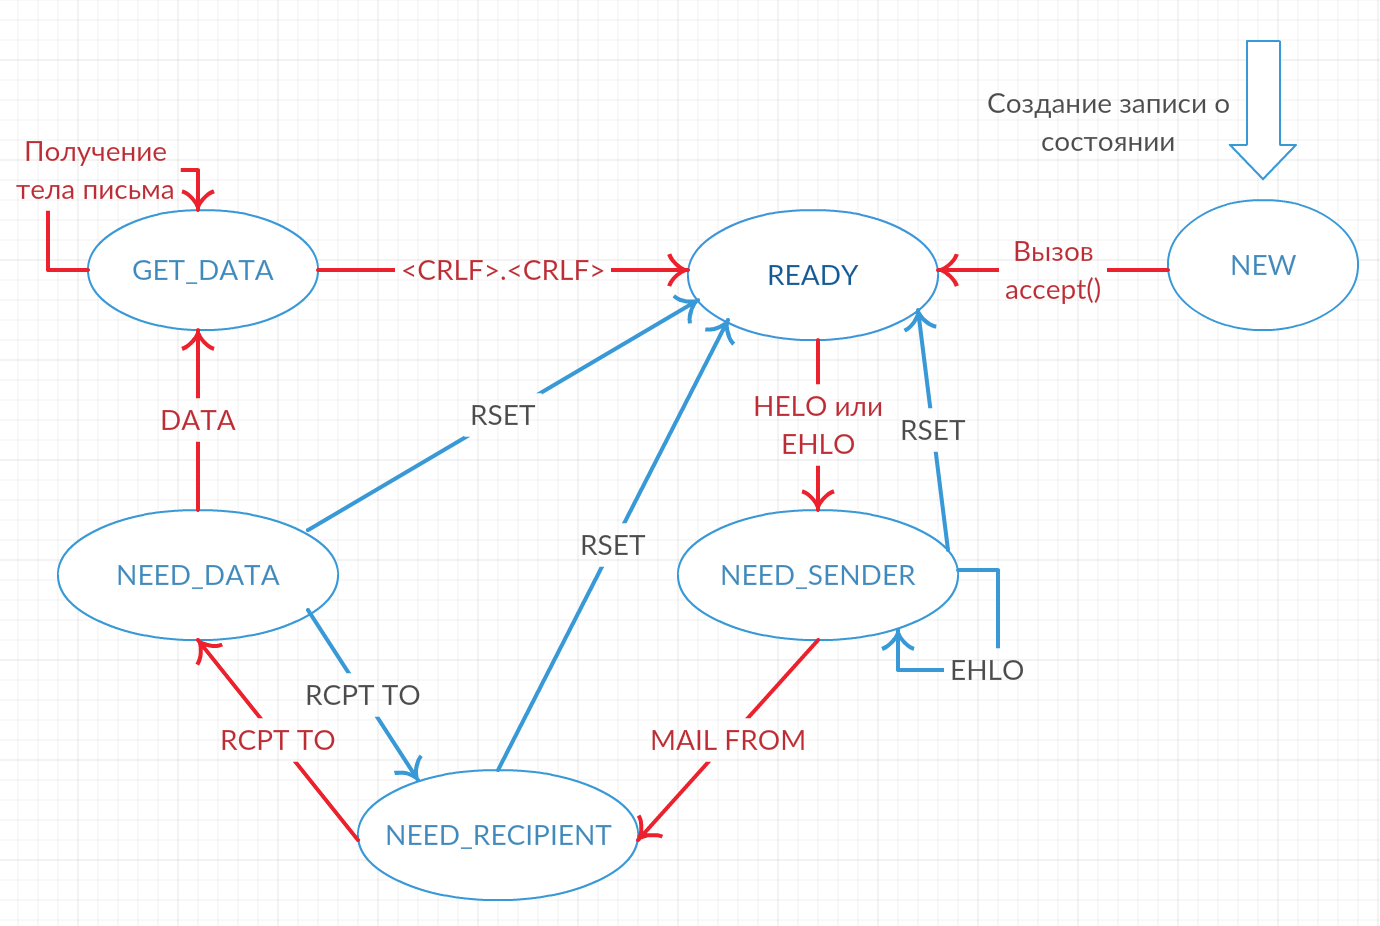
\includegraphics[width=\textwidth]{diagramms/smtp_fsm.png}
\caption{Конечный автомат протокола SMTP}
\label{fig:smtp_fsm}
\end{figure}

На диаграмме красным цветом выделен путь по графу, который соответствует обычной отправке письма с одним получателем. Синим - другие возможные переходы. На диаграмме также не показано несколько команд, которые не меняют состояния - это QUIT (команда серверу о закрытии соединения), NOOP (команда ничего не делать - no operation) и VRFY (доступна для вызова в состояниях READY и NEED_SENDER).

Некоторые из команд используют параметры. Рассмотрим их подробнее:
\begin{itemize}
	\item \textit{HELO domain} и \textit{EHLO domain}, где domain определяется с помощью регулярного выражения \textit{([a-zA-Z0-9]([a-zA-Z0-9\-]{0,61}[a-zA-Z0-9])?\.)+[a-zA-Z]{2,6})}. Команды инициируют smtp-сессию. В ответ на EHLO ожидается развернутый ответ со списком поддерживаемых расширений;
	\item \textit{MAIL FROM: <email>} и \textit{RCPT TO: <email>}, где email определяется с помощью регулярного выражения \textit{([-A-z0-9.]+@([A-z0-9][-A-z0-9]+\.)+[A-z]{2,4})}. Команды задают отправителя и получателя. Получателей может быть несколько.
	\item \textit{VRFY email_part}, где email_part определяется по \textit{([A-z0-9.@-_]+)}. Команда возвращает информацию по известным для сервера пользователям в формате <полное имя> <email>, в email-е которых встретилась передаваемая параметром последовательность символов.
\end{itemize}

На команды клиента сервер отвечает предопределенными в спецификации SMTP кодами. Далее приведем список поддерживаемых команд.
\begin{itemize}
	\item 221 Closing transmission channel - закрытие соединения по инициативе сервера;
	\item 250 OK - команда корректна и принята к исполнению;
	\item 354 Start mail input; end with <CRLF>.<CRLF> - ответ при переходе в состояние GET_DATA;
	\item 451 Requested action aborted: error in processing - ошибки при выполнении дисковых операций с maildir;
	\item 455 Server unable to accommodate parameters - возвращается в случае, когда получателей больше максимума;
	\item 500 Invalid command - неизвестная команда SMTP;
	\item 501 Invalid argument - отсутствие или некорректный аргумент в команде;
	\item 503 Bad sequence of commands - неожиданная команда для текущего состояния;
	\item 550 Sender unknown - email отправителя не является известным для smtp-сервера (известные записаны в файле usersinfo.txt);
	\item 552 Requested mail action aborted: exceeded storage allocation - ошибка выделения памяти, например для тела письма;
\end{itemize}

% \begin{description} \item[Команда выхода из сеанса] \input{include/re_cmd_quit_re.tex} \item[Команда передачи имени пользователя] \input{include/re_cmd_user_re.tex} \end{description}

% Для грамматики можно использовать вставку из файла и оформление \textbackslash{}begin\{verbatim\} и \textbackslash{}end\{verbatim\} или пакет \textit{listings}\footnote{На дворе XXI век, но пакет \textit{listings} всё ещё не пашет с русскими комментариями без бубна, и лично я его пока не победил.}.

% Для примера воспользуемся автоматической вставкой файла описания параметров программы (не забудьте перенести это в технологический раздел) через утилитку \textit{src2tex}.

% \input{include/checkoptn.def.tex} \lstset{language=C} \lstinputlisting{../src/checkoptn.def}

\section{Работа с Maildir}

\section{Логирование в отдельном процессе}


\chapter{Технологический раздел}

% Нужно отметьть, что символ <<\_>> необходимо оформлять как <<\textbackslash\_>>.

\section{Конфигурация в отдельном файле}

\section{Автоматические тесты}

\section{Сборка программы}

% Сборка программы описана в файле \textit{Makefile} системы сборки \textit{make}. Рис.~\ref{fig:make} нагенерили самодельные \textit{makesimple} и \textit{makefile2dot}, а также \textit{dot2tex} и \textit{dot}.

% \begin{figure} \centering \includegraphics[width=\textwidth]{include/Makefile_1_dot.pdf} \caption{Сборка программы} \label{fig:make} \end{figure}

% Отмечу, что за исключения целей типа \textit{all}, \textit{install}, \textit{clean}, \textit{tests}, все имена целей в файле систем сборки \textit{make} обычно совпадают с именами файлов (такой вот низкоуровневый инструмент). То есть вместо цели \textit{lexer} следует использовать цель \textit{src/lexer.c}.

\addcontentsline{toc}{chapter}{Выводы}
\chapter*{Выводы}

Результаты, что сделано и что выполнено.


\cleardoublepage
\phantomsection
\addcontentsline{toc}{chapter}{Приложение 1. Основные функции программы}
\chapter*{Приложение 1. Основные функции программы}

% Весь это раздел сгеренерировал doxygen из части комментированных исходников программы. В файле конфигурации \textbf{doxyggen.cfg} был отключён параметр \textbf{HAVE\_DOT}, поскольку для рисования графов вызовов используется \textit{cflow}.

% \input{include/files}

% \input{include/server-state_8h.tex}
% \input{include/server-state_8c.tex}
% \input{include/server-re_8h.tex}
% \input{include/server-cmd_8h.tex}
% \input{include/server-cmd_8c.tex}
% \input{include/server-parse_8h.tex}
% \input{include/server-parse_8c.tex}
% \input{include/server-run_8h.tex}
% \input{include/server-run_8c.tex}
% \input{include/server_8c.tex}


\cleardoublepage
\phantomsection
\addcontentsline{toc}{chapter}{Приложение 2. Графы вызова функций}
\chapter*{Приложение 2. Графы вызова функций}

% Поскольку функций много, графы вызовов разбиты на два рисунка. На рис.~\ref{fig:cflow01} показаны основные функции, на рис.~\ref{fig:cflow02}~-- функции обработки команд. Файл \textbf{cflow.ignore} содержит список функций (точнее, шабловнов поиска), использыемых программой \textit{grep} для удаления малоинтересных стандартных функций\footnote{Функции по работе с сокетами, ipc и привилегиями к малоинтересным ни в коем случае не относятся.}.

% \begin{figure} \centering \includegraphics[width=\textwidth]{include/cflow01_dot.pdf} \caption{Граф вызовов, основные функции} \label{fig:cflow01} \end{figure}

% \begin{figure} \centering \includegraphics[width=\textwidth]{include/cflow02_dot.pdf} \caption{Граф вызовов, функции обработки команд} \label{fig:cflow02} \end{figure}

% Графы созданы с помощью \textit{cflow}, \textit{cflow2dot}, \textit{dot}.

\end{document}
